\documentclass[aspectratio=169, 10pt]{beamer}

% --- Packages ---
\usepackage[utf8]{inputenc}
\usepackage{tikz}
\usepackage{pgfplots}
\usepackage{amsmath, amssymb, amsfonts}
\usepackage{booktabs}
\usepackage{bm}
\usepackage{xcolor}
\usetikzlibrary{arrows.meta, calc, positioning, shapes.geometric, decorations.pathreplacing, backgrounds, fit, shadows, patterns, shapes.arrows, angles, quotes, decorations.markings}
\pgfplotsset{compat=1.17}

% NYU Colors
\definecolor{nyupurple}{RGB}{87,46,140}
\definecolor{nyuheader}{RGB}{172,159,195}
\definecolor{nyufooter}{RGB}{189,178,211}

% Theme
\usetheme{default}
\setbeamertemplate{navigation symbols}{}

% Itemize
\setbeamercolor{itemize item}{fg=nyupurple}
\setbeamercolor{itemize subitem}{fg=nyupurple}
\setbeamercolor{itemize subsubitem}{fg=nyupurple}
\setbeamertemplate{itemize item}{\textbullet}
\setbeamertemplate{itemize subitem}{\textbullet}
\setbeamertemplate{itemize subsubitem}{\textbullet}

% Blocks
\setbeamercolor{block title}{fg=white, bg=nyupurple}
\setbeamercolor{block body}{fg=black, bg=nyuheader!30}
\setbeamercolor{block title alerted}{fg=white, bg=red!70}
\setbeamercolor{block body alerted}{fg=black, bg=red!10}
\setbeamercolor{block title example}{fg=white, bg=green!50!black}
\setbeamercolor{block body example}{fg=black, bg=green!10}

% Diagram colors
\definecolor{darkblue}{RGB}{0,51,102}
\definecolor{brightblue}{RGB}{0,102,204}
\definecolor{lightblue}{RGB}{153,204,255}
\definecolor{darkgreen}{RGB}{0,102,51}
\definecolor{accentred}{RGB}{192,0,0}
\definecolor{accentgreen}{RGB}{0,128,0}
\definecolor{accentorange}{RGB}{255,128,0}

% Commands
\newcommand{\vect}[1]{\boldsymbol{#1}}
\newcommand{\mat}[1]{\mathbf{#1}}

% Header
\makeatletter
\setbeamertemplate{frametitle}{%
    \nointerlineskip%
    \begin{beamercolorbox}[wd=\paperwidth,ht=0.7cm,dp=0.15cm,rightskip=0.5cm]{frametitle}
        \hspace{0.3cm}\usebeamerfont{frametitle}\insertframetitle%
        \hfill%
        \raisebox{0.08cm}{{\bfseries\sffamily\color{nyupurple}NYU}}%
    \end{beamercolorbox}%
}
\makeatother
\setbeamercolor{frametitle}{fg=black, bg=nyuheader}
\setbeamerfont{frametitle}{size=\large}

% Footer
\setbeamertemplate{footline}{%
    \begin{tikzpicture}[remember picture, overlay]
        \fill[nyufooter] ([yshift=0.6cm]current page.south west) rectangle ([xshift=5cm]current page.south east);
        \fill[nyufooter!70] ([yshift=0.6cm, xshift=5cm]current page.south west) rectangle ([xshift=10.5cm]current page.south east);
        \fill[nyufooter!40] ([yshift=0.6cm, xshift=10.5cm]current page.south west) rectangle (current page.south east);
        \node[anchor=west, font=\small] at ([xshift=0.3cm, yshift=0.3cm]current page.south west) {Dr.\ Aliasghar Arab};
        \node[anchor=center, font=\small] at ([yshift=0.3cm]current page.south) {Autonomous Mobile Robots};
        \node[anchor=east, font=\small] at ([xshift=-0.3cm, yshift=0.3cm]current page.south east) {LECTURE 5 -- FALL 2025 \quad \insertframenumber{} / \inserttotalframenumber};
    \end{tikzpicture}%
}

% Title page
\defbeamertemplate*{title page}{customized}[1][]
{
    \begin{tikzpicture}[remember picture, overlay]
        \node[anchor=north east] at ([xshift=-0.8cm, yshift=-0.8cm]current page.north east) {%
            {\bfseries\sffamily\Large\color{nyupurple}NYU}%
            {\sffamily\normalsize\color{black}\ \ TANDON SCHOOL OF ENGINEERING}%
        };
    \end{tikzpicture}
    
    \vspace{2cm}
    \centering
    {\Large\bfseries\inserttitle\par}
    \vspace{0.3cm}
    {\insertsubtitle\par}
    \vspace{1cm}
    {\insertauthor\par}
    \vspace{0.3cm}
    {\small\insertinstitute\par}
    \vspace{0.5cm}
    {\insertdate\par}
}

% Title info
\title{Autonomous Mobile Robots}
\subtitle{Lecture 5: Lyapunov Stability and Nonlinear Systems}
\author{Dr.\ Aliasghar Arab}
\institute{NYU Tandon School of Engineering}
\date{Fall 2025}

\begin{document}

% ============================================================
% TITLE SLIDE
% ============================================================
{
\setbeamertemplate{footline}{}
\begin{frame}[plain]
\titlepage
\end{frame}
}

% ============================================================
% OVERVIEW
% ============================================================
\begin{frame}{Lecture Overview}

\begin{itemize}
    \item[\textbullet] Nonlinear Systems Fundamentals
    
    \vspace{0.4cm}
    
    \item[\textbullet] Phase Portrait Analysis
    
    \vspace{0.4cm}
    
    \item[\textbullet] Eigenvalue-Based Stability Classification
    
    \vspace{0.4cm}
    
    \item[\textbullet] Lyapunov Stability Theory
    
    \vspace{0.4cm}
    
    \item[\textbullet] Lyapunov Function Examples
    
    \vspace{0.4cm}
    
    \item[\textbullet] Linearization for Stability Analysis
    
    \vspace{0.4cm}
    
    \item[\textbullet] Lyapunov-Based Controller Design
\end{itemize}

\end{frame}

% ============================================================
% SECTION: NONLINEAR SYSTEMS FUNDAMENTALS
% ============================================================
\begin{frame}{Course Topics}

\begin{center}
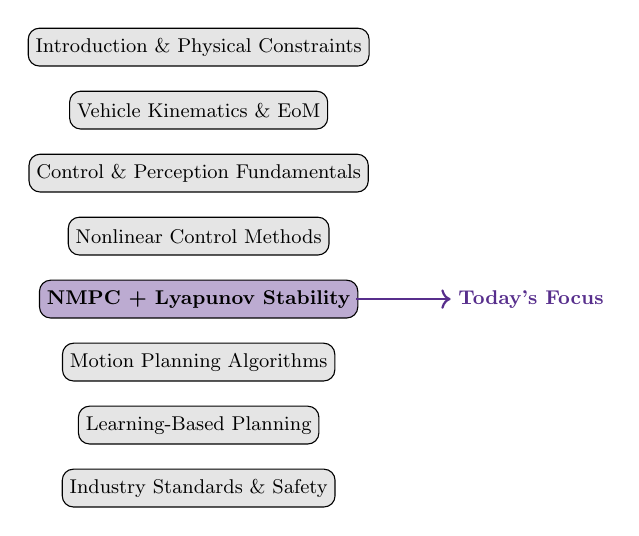
\begin{tikzpicture}[scale=0.8, transform shape]
    \node[draw, rounded corners, fill=gray!20, minimum width=3.5cm, minimum height=0.6cm, font=\small] at (0,4) {Introduction \& Physical Constraints};
    \node[draw, rounded corners, fill=gray!20, minimum width=3.5cm, minimum height=0.6cm, font=\small] at (0,3) {Vehicle Kinematics \& EoM};
    \node[draw, rounded corners, fill=gray!20, minimum width=3.5cm, minimum height=0.6cm, font=\small] at (0,2) {Control \& Perception Fundamentals};
    \node[draw, rounded corners, fill=gray!20, minimum width=3.5cm, minimum height=0.6cm, font=\small] at (0,1) {Nonlinear Control Methods};
    \node[draw, rounded corners, fill=nyupurple!40, minimum width=3.5cm, minimum height=0.6cm, font=\small\bfseries] at (0,0) {NMPC + Lyapunov Stability};
    \node[draw, rounded corners, fill=gray!20, minimum width=3.5cm, minimum height=0.6cm, font=\small] at (0,-1) {Motion Planning Algorithms};
    \node[draw, rounded corners, fill=gray!20, minimum width=3.5cm, minimum height=0.6cm, font=\small] at (0,-2) {Learning-Based Planning};
    \node[draw, rounded corners, fill=gray!20, minimum width=3.5cm, minimum height=0.6cm, font=\small] at (0,-3) {Industry Standards \& Safety};
    
    \draw[->, thick, nyupurple] (2.5,0) -- (4,0);
    \node[right, font=\small\bfseries, nyupurple] at (4,0) {Today's Focus};
\end{tikzpicture}
\end{center}

\end{frame}

% ============================================================
\begin{frame}{Nonlinear Systems: Autonomous Form}

\textbf{Autonomous System} (time-independent):

\vspace{0.5cm}

\begin{equation*}
\dot{X} = f(X)
\end{equation*}

\vspace{0.5cm}

This is a \textbf{closed-loop equation} where dynamics depend only on the current state.

\vspace{0.5cm}

The system evolves independently of explicit time $t$.

\end{frame}

% ============================================================
\begin{frame}{Nonlinear Systems: Non-Autonomous Form}

\textbf{Non-Autonomous System} (with control input):

\vspace{0.5cm}

\begin{equation*}
\dot{X} = f(X, u)
\end{equation*}

\vspace{0.5cm}

With state feedback control $u = g(x)$:

\vspace{0.3cm}

\begin{equation*}
\dot{X} = f(X, g(X))
\end{equation*}

\vspace{0.5cm}

This transforms the non-autonomous system into an autonomous closed-loop system.

\end{frame}

% ============================================================
\begin{frame}{Key Insight: Equilibrium Points}

\begin{block}{Fundamental Difference}
For nonlinear systems, we study behavior \textbf{from equilibrium point to equilibrium point}.
\end{block}

\vspace{0.5cm}

Unlike linear systems with typically one equilibrium, nonlinear systems can have:

\vspace{0.3cm}

\begin{itemize}
    \item[\textbullet] Multiple equilibrium points
    
    \vspace{0.3cm}
    
    \item[\textbullet] Different stability properties at each equilibrium
    
    \vspace{0.3cm}
    
    \item[\textbullet] Complex behaviors between equilibria
\end{itemize}

\end{frame}

% ============================================================
\begin{frame}{Linear vs.\ Nonlinear Systems}

\begin{columns}[T]
\column{0.48\textwidth}
\textbf{Linear Systems}

\vspace{0.3cm}

\begin{itemize}
    \item[\textbullet] Single equilibrium point
    
    \vspace{0.3cm}
    
    \item[\textbullet] Predictable behavior
    
    \vspace{0.3cm}
    
    \item[\textbullet] Global stability analysis
    
    \vspace{0.3cm}
    
    \item[\textbullet] Superposition applies
\end{itemize}

\column{0.48\textwidth}
\textbf{Nonlinear Systems}

\vspace{0.3cm}

\begin{itemize}
    \item[\textbullet] Multiple equilibrium points
    
    \vspace{0.3cm}
    
    \item[\textbullet] Chaos, bifurcations
    
    \vspace{0.3cm}
    
    \item[\textbullet] Local stability only
    
    \vspace{0.3cm}
    
    \item[\textbullet] No superposition
\end{itemize}
\end{columns}

\end{frame}

% ============================================================
\begin{frame}{Important Limitation of Linearization}

\begin{alertblock}{Critical Note}
Linearization gives only \textbf{local information} at each equilibrium point $\dot{x} = 0$.
\end{alertblock}

\vspace{0.5cm}

It tells us nothing about:

\vspace{0.3cm}

\begin{itemize}
    \item[\textbullet] Global behavior of the system
    
    \vspace{0.3cm}
    
    \item[\textbullet] Behavior far from the equilibrium
    
    \vspace{0.3cm}
    
    \item[\textbullet] Interactions between multiple equilibria
\end{itemize}

\end{frame}

% ============================================================
% SECTION: PHASE PORTRAIT ANALYSIS
% ============================================================
\begin{frame}{Methods to Analyze Nonlinear Systems}

\textbf{Phase Portrait Analysis}

\vspace{0.5cm}

Plotting trajectories in state space helps visualize system behavior.

\vspace{0.5cm}

\begin{itemize}
    \item[\textbullet] Shows how states evolve over time
    
    \vspace{0.3cm}
    
    \item[\textbullet] Reveals equilibrium points and their stability
    
    \vspace{0.3cm}
    
    \item[\textbullet] Identifies limit cycles and attractors
\end{itemize}

\vspace{0.5cm}

\textbf{Limitation:} Can be used at most for 2nd-order differential equations (2D state space).

\end{frame}

% ============================================================
\begin{frame}{Example: Linear 2nd-Order System}

\textbf{General Linear Oscillator:}

\vspace{0.5cm}

\begin{equation*}
\ddot{y} + 2\varepsilon \omega_n \dot{y} + \omega_n^2 y = 0
\end{equation*}

\vspace{0.5cm}

where:

\vspace{0.3cm}

\begin{itemize}
    \item[\textbullet] $\varepsilon$ = damping ratio
    
    \vspace{0.3cm}
    
    \item[\textbullet] $\omega_n$ = natural frequency
\end{itemize}

\end{frame}

% ============================================================
\begin{frame}{Converting to State-Space Form}

\textbf{Define state variables:}

\vspace{0.4cm}

\begin{equation*}
X_1 = y \qquad X_2 = \dot{y} \qquad X = \begin{bmatrix} X_1 \\ X_2 \end{bmatrix}
\end{equation*}

\vspace{0.5cm}

\textbf{State equations:}

\vspace{0.4cm}

\begin{align*}
\dot{X}_1 &= X_2 \\[0.3cm]
\dot{X}_2 &= -\omega_n^2 X_1 - 2\varepsilon \omega_n X_2
\end{align*}

\end{frame}

% ============================================================
\begin{frame}{Matrix Form}

\textbf{State-space representation:}

\vspace{0.5cm}

\begin{equation*}
\dot{X} = AX
\end{equation*}

\vspace{0.5cm}

\begin{equation*}
A = \begin{bmatrix} 0 & 1 \\ -\omega_n^2 & -2\varepsilon \omega_n \end{bmatrix}
\end{equation*}

\end{frame}

% ============================================================
\begin{frame}{Finding Equilibrium Points}

\textbf{Equilibrium condition:}

\vspace{0.5cm}

\begin{equation*}
\dot{X} = 0 \quad \Rightarrow \quad X^* = 0
\end{equation*}

\vspace{0.5cm}

For this linear system, \textbf{the origin is the only equilibrium point}.

\vspace{0.5cm}

The stability of this equilibrium depends on the eigenvalues of matrix $A$.

\end{frame}

% ============================================================
% SECTION: EIGENVALUE STABILITY CLASSIFICATION
% ============================================================
\begin{frame}{Stability Classification via Eigenvalues}

System behavior is determined by eigenvalues $\lambda_1, \lambda_2$ of matrix $A$.

\vspace{0.5cm}

\textbf{Key factors:}

\vspace{0.3cm}

\begin{itemize}
    \item[\textbullet] Real part: $\text{Re}\{\lambda\}$ determines growth/decay
    
    \vspace{0.3cm}
    
    \item[\textbullet] Imaginary part: $\text{Im}\{\lambda\}$ determines oscillation
\end{itemize}

\vspace{0.5cm}

Let's examine each case with phase portraits.

\end{frame}

% ============================================================
\begin{frame}{Case 1: Stable Node}

\begin{columns}[T]
\column{0.45\textwidth}
\textbf{Eigenvalue Conditions:}

\vspace{0.4cm}

\begin{equation*}
\text{Re}\{\lambda_1, \lambda_2\} < 0
\end{equation*}

\vspace{0.3cm}

\begin{equation*}
\text{Im}\{\lambda_1, \lambda_2\} = 0
\end{equation*}

\vspace{0.5cm}

Both eigenvalues are \textbf{real and negative}.

\vspace{0.3cm}

$\Rightarrow$ \textbf{Stable Equilibrium}

\column{0.52\textwidth}
\begin{center}
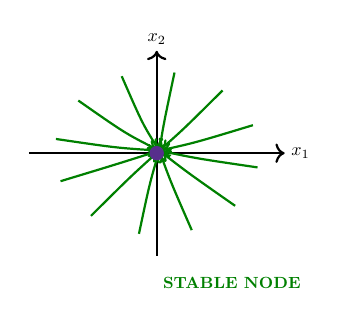
\begin{tikzpicture}[scale=0.65, transform shape]
    \draw[->, thick] (-2.5,0) -- (2.5,0) node[right] {$x_1$};
    \draw[->, thick] (0,-2) -- (0,2) node[above] {$x_2$};
    
    % Trajectories converging to origin
    \foreach \angle in {20,50,80,110,140,170,200,230,260,290,320,350} {
        \draw[->, accentgreen, thick] ({2*cos(\angle)},{1.6*sin(\angle)}) 
            .. controls ({0.8*cos(\angle)},{0.6*sin(\angle)}) .. (0.05,0.05);
    }
    
    \fill[nyupurple] (0,0) circle (4pt);
    \node[below right, font=\small\bfseries, accentgreen] at (0,-2.3) {STABLE NODE};
\end{tikzpicture}
\end{center}
\end{columns}

\end{frame}

% ============================================================
\begin{frame}{Case 2: Stable Focus (Spiral)}

\begin{columns}[T]
\column{0.45\textwidth}
\textbf{Eigenvalue Conditions:}

\vspace{0.4cm}

\begin{equation*}
\text{Re}\{\lambda_1, \lambda_2\} < 0
\end{equation*}

\vspace{0.3cm}

\begin{equation*}
\text{Im}\{\lambda_1, \lambda_2\} \neq 0
\end{equation*}

\vspace{0.5cm}

Complex conjugate eigenvalues with negative real part.

\vspace{0.3cm}

$\Rightarrow$ \textbf{Stable Spiral}

\column{0.52\textwidth}
\begin{center}
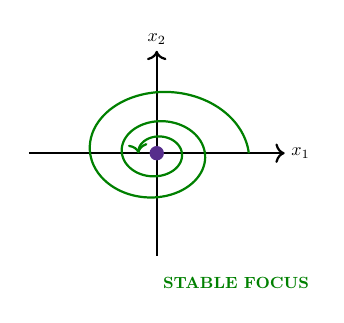
\begin{tikzpicture}[scale=0.65, transform shape]
    \draw[->, thick] (-2.5,0) -- (2.5,0) node[right] {$x_1$};
    \draw[->, thick] (0,-2) -- (0,2) node[above] {$x_2$};
    
    % Spiral inward
    \draw[->, accentgreen, thick, domain=0:900, samples=200, smooth] 
        plot ({1.8*exp(-0.0018*\x)*cos(\x)}, {1.4*exp(-0.0018*\x)*sin(\x)});
    
    \fill[nyupurple] (0,0) circle (4pt);
    \node[below right, font=\small\bfseries, accentgreen] at (0,-2.3) {STABLE FOCUS};
\end{tikzpicture}
\end{center}
\end{columns}

\end{frame}

% ============================================================
\begin{frame}{Case 3: Unstable Node (Source)}

\begin{columns}[T]
\column{0.45\textwidth}
\textbf{Eigenvalue Conditions:}

\vspace{0.4cm}

\begin{equation*}
\text{Re}\{\lambda_1, \lambda_2\} < 0
\end{equation*}

\vspace{0.3cm}

\begin{equation*}
\text{Im}\{\lambda_1, \lambda_2\} = 0
\end{equation*}

\vspace{0.5cm}

\textbf{Note:} Despite $\text{Re} < 0$ shown, if signs were positive, trajectories diverge.

\vspace{0.3cm}

This is an \textbf{Unstable Equilibrium} --- stable only at exactly $x^* = 0$.

\column{0.52\textwidth}
\begin{center}
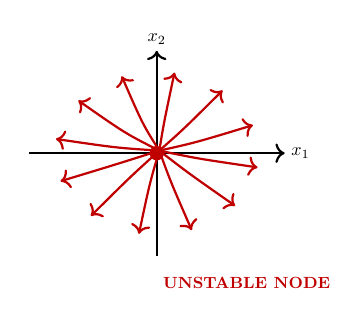
\begin{tikzpicture}[scale=0.65, transform shape]
    \draw[->, thick] (-2.5,0) -- (2.5,0) node[right] {$x_1$};
    \draw[->, thick] (0,-2) -- (0,2) node[above] {$x_2$};
    
    % Trajectories diverging from origin
    \foreach \angle in {20,50,80,110,140,170,200,230,260,290,320,350} {
        \draw[->, accentred, thick] (0.05,0.05) 
            .. controls ({0.8*cos(\angle)},{0.6*sin(\angle)}) .. ({2*cos(\angle)},{1.6*sin(\angle)});
    }
    
    \fill[accentred] (0,0) circle (4pt);
    \node[below right, font=\small\bfseries, accentred] at (0,-2.3) {UNSTABLE NODE};
\end{tikzpicture}
\end{center}
\end{columns}

\end{frame}

% ============================================================
\begin{frame}{Case 4: Unstable Focus}

\begin{columns}[T]
\column{0.45\textwidth}
\textbf{Eigenvalue Conditions:}

\vspace{0.4cm}

\begin{equation*}
\text{Re}\{\lambda_1, \lambda_2\} > 0
\end{equation*}

\vspace{0.3cm}

\begin{equation*}
\text{Im}\{\lambda_1, \lambda_2\} = 0
\end{equation*}

\vspace{0.5cm}

Both eigenvalues are \textbf{real and positive}.

\vspace{0.3cm}

$\Rightarrow$ \textbf{Unstable Equilibrium}

\column{0.52\textwidth}
\begin{center}
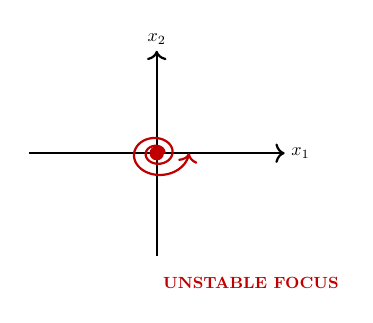
\begin{tikzpicture}[scale=0.65, transform shape]
    \draw[->, thick] (-2.5,0) -- (2.5,0) node[right] {$x_1$};
    \draw[->, thick] (0,-2) -- (0,2) node[above] {$x_2$};
    
    % Spiral outward
    \draw[->, accentred, thick, domain=0:720, samples=200, smooth] 
        plot ({0.15*exp(0.002*\x)*cos(\x)}, {0.12*exp(0.002*\x)*sin(\x)});
    
    \fill[accentred] (0,0) circle (4pt);
    \node[below right, font=\small\bfseries, accentred] at (0,-2.3) {UNSTABLE FOCUS};
\end{tikzpicture}
\end{center}
\end{columns}

\end{frame}

% ============================================================
\begin{frame}{Case 5: Saddle Point}

\begin{columns}[T]
\column{0.45\textwidth}
\textbf{Eigenvalue Conditions:}

\vspace{0.4cm}

\begin{equation*}
\text{Re}\{\lambda_1\} < 0
\end{equation*}

\vspace{0.3cm}

\begin{equation*}
\text{Re}\{\lambda_2\} > 0
\end{equation*}

\vspace{0.5cm}

One stable direction, one unstable direction.

\vspace{0.3cm}

$\Rightarrow$ \textbf{Saddle Point (Unstable)}

\column{0.52\textwidth}
\begin{center}
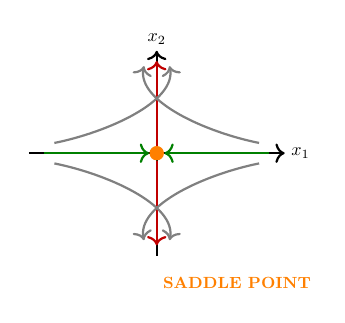
\begin{tikzpicture}[scale=0.65, transform shape]
    \draw[->, thick] (-2.5,0) -- (2.5,0) node[right] {$x_1$};
    \draw[->, thick] (0,-2) -- (0,2) node[above] {$x_2$};
    
    % Stable manifold (horizontal)
    \draw[->, accentgreen, thick] (-2.2,0) -- (-0.15,0);
    \draw[->, accentgreen, thick] (2.2,0) -- (0.15,0);
    
    % Unstable manifold (vertical)
    \draw[->, accentred, thick] (0,0.15) -- (0,1.8);
    \draw[->, accentred, thick] (0,-0.15) -- (0,-1.8);
    
    % Hyperbolic trajectories
    \draw[->, gray, thick] (-2,0.2) .. controls (-1,0.4) and (0.4,1) .. (0.25,1.7);
    \draw[->, gray, thick] (2,0.2) .. controls (1,0.4) and (-0.4,1) .. (-0.25,1.7);
    \draw[->, gray, thick] (-2,-0.2) .. controls (-1,-0.4) and (0.4,-1) .. (0.25,-1.7);
    \draw[->, gray, thick] (2,-0.2) .. controls (1,-0.4) and (-0.4,-1) .. (-0.25,-1.7);
    
    \fill[accentorange] (0,0) circle (4pt);
    \node[below right, font=\small\bfseries, accentorange] at (0,-2.3) {SADDLE POINT};
\end{tikzpicture}
\end{center}
\end{columns}

\end{frame}

% ============================================================
\begin{frame}{Case 6: Center (Marginally Stable)}

\begin{columns}[T]
\column{0.45\textwidth}
\textbf{Eigenvalue Conditions:}

\vspace{0.4cm}

\begin{equation*}
\text{Re}\{\lambda_1, \lambda_2\} = 0
\end{equation*}

\vspace{0.3cm}

\begin{equation*}
\text{Im}\{\lambda_1, \lambda_2\} \neq 0
\end{equation*}

\vspace{0.5cm}

Purely imaginary eigenvalues.

\vspace{0.3cm}

Example: Spring-damper with no damping.

\column{0.52\textwidth}
\begin{center}
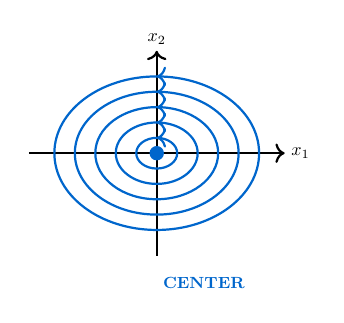
\begin{tikzpicture}[scale=0.65, transform shape]
    \draw[->, thick] (-2.5,0) -- (2.5,0) node[right] {$x_1$};
    \draw[->, thick] (0,-2) -- (0,2) node[above] {$x_2$};
    
    % Concentric ellipses
    \foreach \r in {0.4,0.8,1.2,1.6,2.0} {
        \draw[brightblue, thick, decoration={markings, mark=at position 0.25 with {\arrow{>}}}, postaction={decorate}] 
            (0,0) ellipse ({\r} and {0.75*\r});
    }
    
    \fill[brightblue] (0,0) circle (4pt);
    \node[below right, font=\small\bfseries, brightblue] at (0,-2.3) {CENTER};
\end{tikzpicture}
\end{center}
\end{columns}

\end{frame}

% ============================================================
\begin{frame}{Summary: Eigenvalue Stability Classification}

\begin{center}
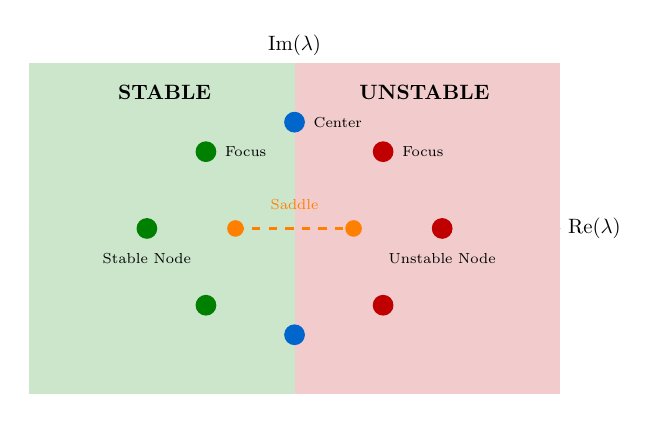
\begin{tikzpicture}[scale=0.75, transform shape]
    % Complex plane
    \draw[->, thick] (-4.5,0) -- (4.5,0) node[right] {$\text{Re}(\lambda)$};
    \draw[->, thick] (0,-2.8) -- (0,2.8) node[above] {$\text{Im}(\lambda)$};
    
    % Regions
    \fill[accentgreen!20] (-4.5,-2.8) rectangle (0,2.8);
    \fill[accentred!20] (0,-2.8) rectangle (4.5,2.8);
    
    % Labels
    \node[font=\bfseries] at (-2.2,2.3) {STABLE};
    \node[font=\bfseries] at (2.2,2.3) {UNSTABLE};
    
    % Points
    \fill[accentgreen] (-2.5,0) circle (5pt);
    \node[below, font=\scriptsize] at (-2.5,-0.3) {Stable Node};
    
    \fill[accentgreen] (-1.5,1.3) circle (5pt);
    \fill[accentgreen] (-1.5,-1.3) circle (5pt);
    \node[right, font=\scriptsize] at (-1.3,1.3) {Focus};
    
    \fill[accentred] (2.5,0) circle (5pt);
    \node[below, font=\scriptsize] at (2.5,-0.3) {Unstable Node};
    
    \fill[accentred] (1.5,1.3) circle (5pt);
    \fill[accentred] (1.5,-1.3) circle (5pt);
    \node[right, font=\scriptsize] at (1.7,1.3) {Focus};
    
    \fill[brightblue] (0,1.8) circle (5pt);
    \fill[brightblue] (0,-1.8) circle (5pt);
    \node[right, font=\scriptsize] at (0.2,1.8) {Center};
    
    % Saddle
    \fill[accentorange] (-1,0) circle (4pt);
    \fill[accentorange] (1,0) circle (4pt);
    \draw[accentorange, thick, dashed] (-1,0) -- (1,0);
    \node[above, font=\scriptsize, accentorange] at (0,0.2) {Saddle};
\end{tikzpicture}
\end{center}

\end{frame}

% ============================================================
% SECTION: NONLINEAR SYSTEM EXAMPLES
% ============================================================
\begin{frame}{Nonlinear System Example}

\textbf{Cubic Damping System:}

\vspace{0.5cm}

\begin{equation*}
\ddot{x} + \alpha \dot{x} + x^3 = 0
\end{equation*}

\vspace{0.5cm}

\begin{itemize}
    \item[\textbullet] Nonlinear restoring force: $x^3$
    
    \vspace{0.3cm}
    
    \item[\textbullet] Linear damping: $\alpha \dot{x}$
    
    \vspace{0.3cm}
    
    \item[\textbullet] Stiffness increases with displacement
\end{itemize}

\end{frame}

% ============================================================
\begin{frame}{Nonlinear System: Phase Portrait}

\begin{center}
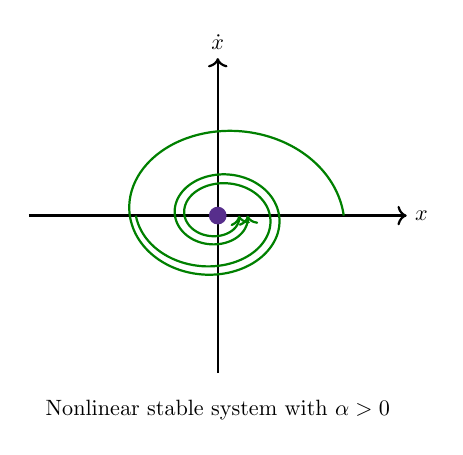
\begin{tikzpicture}[scale=0.8, transform shape]
    \draw[->, thick] (-3,0) -- (3,0) node[right] {$x$};
    \draw[->, thick] (0,-2.5) -- (0,2.5) node[above] {$\dot{x}$};
    
    % Spiral trajectories inward
    \draw[->, accentgreen, thick, domain=0:720, samples=200, smooth] 
        plot ({2*exp(-0.002*\x)*cos(\x)}, {1.6*exp(-0.002*\x)*sin(\x)});
    
    \draw[->, accentgreen, thick, domain=0:540, samples=150, smooth] 
        plot ({1.3*exp(-0.0025*\x)*cos(\x+180)}, {1*exp(-0.0025*\x)*sin(\x+180)});
    
    \fill[nyupurple] (0,0) circle (4pt);
    \node[below] at (0,-2.8) {Nonlinear stable system with $\alpha > 0$};
\end{tikzpicture}
\end{center}

\end{frame}

% ============================================================
\begin{frame}{Nonlinear System: Switching Model}

\textbf{Satellite Attitude Control (Bang-Bang):}

\vspace{0.5cm}

\begin{equation*}
\ddot{\theta} = K \cdot \text{sign}(-\theta)
\end{equation*}

\vspace{0.5cm}

\begin{itemize}
    \item[\textbullet] Used in spacecraft attitude control
    
    \vspace{0.3cm}
    
    \item[\textbullet] Discontinuous control input
    
    \vspace{0.3cm}
    
    \item[\textbullet] Can achieve finite-time convergence
\end{itemize}

\end{frame}

% ============================================================
\begin{frame}{Switching Model: Phase Portrait}

\begin{center}
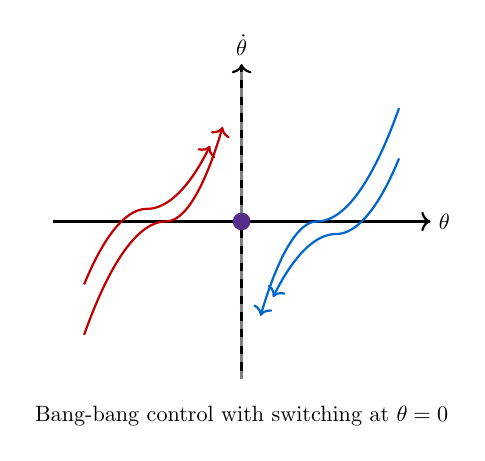
\begin{tikzpicture}[scale=0.8, transform shape]
    \draw[->, thick] (-3,0) -- (3,0) node[right] {$\theta$};
    \draw[->, thick] (0,-2.5) -- (0,2.5) node[above] {$\dot{\theta}$};
    
    % Right half: parabolas going left
    \draw[->, brightblue, thick] (2.5,1.8) parabola bend (1.2,0) (0.3,-1.5);
    \draw[->, brightblue, thick] (2.5,1) parabola bend (1.5,-0.2) (0.5,-1.2);
    
    % Left half: parabolas going right
    \draw[->, accentred, thick] (-2.5,-1.8) parabola bend (-1.2,0) (-0.3,1.5);
    \draw[->, accentred, thick] (-2.5,-1) parabola bend (-1.5,0.2) (-0.5,1.2);
    
    % Switching line
    \draw[dashed, thick, gray] (0,-2.5) -- (0,2.5);
    
    \fill[nyupurple] (0,0) circle (4pt);
    \node[below] at (0,-2.8) {Bang-bang control with switching at $\theta = 0$};
\end{tikzpicture}
\end{center}

\end{frame}

% ============================================================
% SECTION: LYAPUNOV STABILITY THEORY
% ============================================================
\begin{frame}{Lyapunov Stability: Definition}

\begin{block}{Lyapunov Stability}
An equilibrium $x^* = 0$ is \textbf{Lyapunov stable} if:
\end{block}

\vspace{0.5cm}

\begin{equation*}
\forall R > 0, \; \exists r > 0: \quad \|x(0)\| < r \;\Rightarrow\; \|x(t)\| < R \quad \forall t \geq 0
\end{equation*}

\vspace{0.5cm}

\textbf{Intuition:} Starting close to equilibrium means staying close.

\end{frame}

% ============================================================
\begin{frame}{Lyapunov Stability: Visualization}

\begin{center}
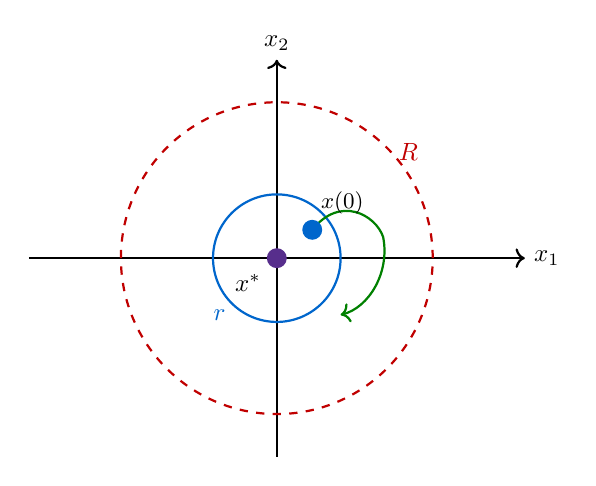
\begin{tikzpicture}[scale=0.9, transform shape]
    \draw[->, thick] (-3.5,0) -- (3.5,0) node[right] {$x_1$};
    \draw[->, thick] (0,-2.8) -- (0,2.8) node[above] {$x_2$};
    
    % Outer ball R
    \draw[accentred, thick, dashed] (0,0) circle (2.2);
    \node[accentred, right] at (1.6,1.5) {$R$};
    
    % Inner ball r
    \draw[brightblue, thick] (0,0) circle (0.9);
    \node[brightblue, below left] at (-0.6,-0.6) {$r$};
    
    % Trajectory staying inside
    \draw[->, accentgreen, thick] (0.5,0.4) .. controls (0.9,0.9) and (1.4,0.6) .. (1.5,0.3) 
        .. controls (1.6,-0.2) and (1.3,-0.7) .. (0.9,-0.8);
    
    % Initial point
    \fill[brightblue] (0.5,0.4) circle (4pt);
    \node[above right, font=\small] at (0.5,0.5) {$x(0)$};
    
    \fill[nyupurple] (0,0) circle (4pt);
    \node[below left] at (-0.1,-0.1) {$x^*$};
\end{tikzpicture}
\end{center}

\end{frame}

% ============================================================
\begin{frame}{Asymptotic Stability}

\begin{block}{Asymptotic Stability}
An equilibrium is \textbf{asymptotically stable} if it is Lyapunov stable AND:
\end{block}

\vspace{0.5cm}

\begin{equation*}
x(t) \to 0 \quad \text{as} \quad t \to \infty
\end{equation*}

\vspace{0.5cm}

\textbf{Key Insight:} Asymptotic stability is \textbf{stronger} than Lyapunov stability.

\vspace{0.3cm}

\begin{itemize}
    \item[\textbullet] Lyapunov stable: stays bounded
    
    \vspace{0.3cm}
    
    \item[\textbullet] Asymptotically stable: converges to equilibrium
\end{itemize}

\end{frame}

% ============================================================
\begin{frame}{Lyapunov Stability Conditions}

For system $\dot{x} = f(x)$ with equilibrium $x^* \Rightarrow \dot{x}^* = 0$:

\vspace{0.5cm}

\begin{block}{Lyapunov's Direct Method}
If there exists a function $V(x)$ such that:

\vspace{0.3cm}

\begin{enumerate}
    \item $V(x) > 0$ for $x \neq 0$ and $V(0) = 0$ \hfill (positive definite)
    
    \vspace{0.3cm}
    
    \item $\dot{V}(x) \leq 0$ for $x \neq 0$ \hfill (non-increasing)
\end{enumerate}

\vspace{0.3cm}

Then the equilibrium is \textbf{Lyapunov stable}.
\end{block}

\end{frame}

% ============================================================
\begin{frame}{Conditions for Asymptotic Stability}

If additionally:

\vspace{0.5cm}

\begin{itemize}
    \item[\textbullet] $\dot{V}(x) = 0$ \textbf{only at} $x = 0$
\end{itemize}

\vspace{0.5cm}

Then $x(t) \to 0$ as $t \to \infty$ $\Rightarrow$ \textbf{Asymptotic stability}

\end{frame}

% ============================================================
\begin{frame}{Global Stability Condition}

For \textbf{global asymptotic stability}, we additionally need:

\vspace{0.5cm}

\begin{equation*}
V(x) \to \infty \quad \text{as} \quad \|x\| \to \infty
\end{equation*}

\vspace{0.5cm}

This is called the \textbf{radially unbounded} condition.

\vspace{0.5cm}

It ensures stability holds for \textit{any} initial condition, not just those near the equilibrium.

\end{frame}

% ============================================================
\begin{frame}{Energy Interpretation of Lyapunov Functions}

\begin{center}
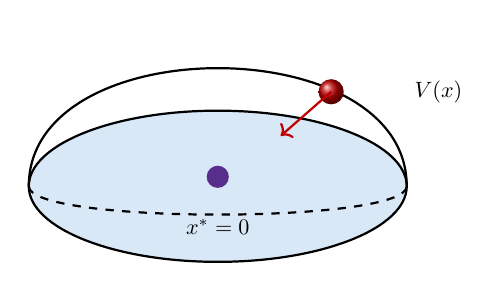
\begin{tikzpicture}[scale=0.8, transform shape]
    % Bowl surface
    \draw[thick, fill=brightblue!15] (0,0) ellipse (3 and 1.2);
    \draw[thick] (-3,0) .. controls (-3,2.5) and (3,2.5) .. (3,0);
    \draw[thick, dashed] (-3,0) .. controls (-3,-0.6) and (3,-0.6) .. (3,0);
    
    % Ball rolling down
    \shade[ball color=accentred] (1.8,1.5) circle (0.2);
    \draw[->, thick, accentred] (1.8,1.5) -- (1,0.8);
    
    % Minimum
    \fill[nyupurple] (0,0.15) circle (5pt);
    \node[below] at (0,-0.4) {$x^* = 0$};
    
    % Label
    \node[right] at (3,1.5) {$V(x)$};
\end{tikzpicture}
\end{center}

\vspace{0.3cm}

$V(x)$ acts like ``energy'' --- if energy always decreases, system approaches minimum.

\end{frame}

% ============================================================
% SECTION: LYAPUNOV EXAMPLES
% ============================================================
\begin{frame}{Example: Nonlinear System}

\textbf{System:}

\vspace{0.4cm}

\begin{equation*}
\ddot{X} + |\dot{X}|\dot{X} + X^3 = 0
\end{equation*}

\vspace{0.5cm}

\textbf{State Variables:}

\vspace{0.3cm}

\begin{equation*}
X_1 = X \qquad X_2 = \dot{X}
\end{equation*}

\end{frame}

% ============================================================
\begin{frame}{Choosing a Lyapunov Function}

\textbf{We choose:}

\vspace{0.5cm}

\begin{equation*}
V(x) = \frac{1}{2}\dot{x}^2 + \frac{1}{4}x^4
\end{equation*}

\vspace{0.5cm}

\textbf{Verification:}

\vspace{0.3cm}

\begin{itemize}
    \item[\textbullet] $V(0) = 0$ \quad \checkmark
    
    \vspace{0.3cm}
    
    \item[\textbullet] $V(x) > 0$ for $x \neq 0$ \quad \checkmark \quad (sum of positive terms)
\end{itemize}

\vspace{0.5cm}

This is a valid \textbf{Lyapunov function candidate}.

\end{frame}

% ============================================================
\begin{frame}{Computing the Time Derivative}

\textbf{Derivative calculation:}

\vspace{0.5cm}

\begin{equation*}
\dot{V}(x) = \ddot{X} \cdot \dot{X} + \dot{X} \cdot X^3 = \dot{X}(\ddot{X} + X^3)
\end{equation*}

\vspace{0.5cm}

\textbf{Substitute from original equation:} $\ddot{X} = -|\dot{X}|\dot{X} - X^3$

\vspace{0.5cm}

\begin{equation*}
\dot{V}(x) = \dot{X}(-|\dot{X}|\dot{X} - X^3 + X^3) = -|\dot{X}|^3
\end{equation*}

\end{frame}

% ============================================================
\begin{frame}{Stability Conclusion}

\textbf{Result:}

\vspace{0.5cm}

\begin{equation*}
\dot{V}(x) = -|\dot{X}|^3 \leq 0
\end{equation*}

\vspace{0.5cm}

Since $\dot{V} \leq 0$, the system is \textbf{Lyapunov stable}.

\vspace{0.5cm}

Since $V(x) \to \infty$ as $\|x\| \to \infty$, it is \textbf{globally stable}.

\vspace{0.5cm}

\begin{block}{Stability Analysis Summary}
Semi-negative definite $\dot{V}$ $\Rightarrow$ Lyapunov stable and globally stable
\end{block}

\end{frame}

% ============================================================
% SECTION: LINEARIZATION
% ============================================================
\begin{frame}{Linearization for Stability Analysis}

\textbf{Nonlinear Equation of Motion:}

\vspace{0.5cm}

\begin{equation*}
\ddot{x} + |\dot{x}|\dot{x} + x + x^3 = 0
\end{equation*}

\vspace{0.5cm}

\textbf{State Variables:}

\vspace{0.3cm}

\begin{equation*}
x_1 = x, \quad x_2 = \dot{x}
\end{equation*}

\vspace{0.5cm}

\textbf{Goal:} Analyze stability at equilibrium $x^* = 0$.

\end{frame}

% ============================================================
\begin{frame}{State-Space Form}

\textbf{System in state-space form:}

\vspace{0.5cm}

\begin{equation*}
\dot{X} = f(X) \quad \text{with} \quad X = \begin{bmatrix} x_1 \\ x_2 \end{bmatrix}^T
\end{equation*}

\vspace{0.5cm}

\begin{align*}
f_1: \quad \dot{x}_1 &= x_2 \\[0.3cm]
f_2: \quad \dot{x}_2 &= -|x_2|x_2 - x_1 - x_1^3
\end{align*}

\end{frame}

% ============================================================
\begin{frame}{Computing the Jacobian Matrix}

\textbf{Jacobian at equilibrium:}

\vspace{0.5cm}

\begin{equation*}
A = \frac{\partial f}{\partial x}\bigg|_{(0,0)}
\end{equation*}

\vspace{0.5cm}

\begin{equation*}
A = \begin{bmatrix} \frac{\partial f_1}{\partial x_1} & \frac{\partial f_1}{\partial x_2} \\[0.3cm] \frac{\partial f_2}{\partial x_1} & \frac{\partial f_2}{\partial x_2} \end{bmatrix} = \begin{bmatrix} 0 & 1 \\ -1 & 0 \end{bmatrix}
\end{equation*}

\end{frame}

% ============================================================
\begin{frame}{Taylor Series Expansion}

\textbf{General linearization formula:}

\vspace{0.5cm}

\begin{equation*}
f(x,u) = f(0,0) + \frac{\partial f}{\partial x}\bigg|_{x=0,u=0} \cdot x + \frac{\partial f}{\partial u}\bigg|_{x=0,u=0} \cdot u + \text{H.O.T.}
\end{equation*}

\vspace{0.5cm}

At equilibrium $(0,0)$:

\vspace{0.3cm}

\begin{equation*}
\dot{x}_2 = -x_1 - 0 \cdot x_2 = -x_1
\end{equation*}

\end{frame}

% ============================================================
\begin{frame}{Eigenvalue Analysis}

\textbf{Characteristic equation:}

\vspace{0.5cm}

\begin{equation*}
\det(\lambda I - A) = \det\begin{bmatrix} \lambda & -1 \\ 1 & \lambda \end{bmatrix} = \lambda^2 + 1 = 0
\end{equation*}

\vspace{0.5cm}

\textbf{Eigenvalues:}

\vspace{0.3cm}

\begin{equation*}
\lambda_{1,2} = \pm i
\end{equation*}

\end{frame}

% ============================================================
\begin{frame}{Stability Conclusion from Linearization}

\textbf{Result:} $\lambda_{1,2} = \pm i$ (purely imaginary)

\vspace{0.5cm}

\begin{alertblock}{Important Caveat}
Linearization at a \textbf{center} is inconclusive!
\end{alertblock}

\vspace{0.3cm}

\begin{itemize}
    \item[\textbullet] Linear analysis suggests center (marginally stable)
    
    \vspace{0.3cm}
    
    \item[\textbullet] Nonlinear terms determine actual stability
    
    \vspace{0.3cm}
    
    \item[\textbullet] Must use Lyapunov analysis for definitive answer
\end{itemize}

\end{frame}

% ============================================================
% SECTION: CHOOSING LYAPUNOV FUNCTIONS
% ============================================================
\begin{frame}{Three Main Methods for Choosing $V(x)$}

\textbf{1. Energy Interpretation:}

\vspace{0.3cm}

Any scalar function that mirrors system energy.

\vspace{0.5cm}

\textbf{2. Sum of Squares Method:}

\vspace{0.3cm}

\begin{equation*}
V(x) = F(x)^T F(x)
\end{equation*}

\vspace{0.5cm}

\textbf{3. Quadratic Form (Linear Systems):}

\vspace{0.3cm}

\begin{equation*}
V(x) = x^T P x
\end{equation*}

where $P$ is positive definite.

\end{frame}

% ============================================================
\begin{frame}{Simple Lyapunov Function Choices}

\textbf{General quadratic form:}

\vspace{0.5cm}

\begin{equation*}
V(x) = \frac{1}{2}x^T x
\end{equation*}

\vspace{0.5cm}

\textbf{For linear systems $\dot{x} = Ax$:}

\vspace{0.5cm}

\begin{equation*}
V = x^T P x
\end{equation*}

\vspace{0.3cm}

where $P$ solves the Lyapunov equation: $A^T P + PA = -Q$ for positive definite $Q$.

\end{frame}

% ============================================================
% SECTION: LYAPUNOV-BASED CONTROL
% ============================================================
\begin{frame}{Designing a Lyapunov-Based Controller}

\textbf{Problem:} Given $\dot{X} = f(x, u)$

\vspace{0.5cm}

\textbf{Goal:} Find $u^*(t)$ such that $x(0) \to x_d$ as $t \to \infty$

\vspace{0.5cm}

\begin{center}
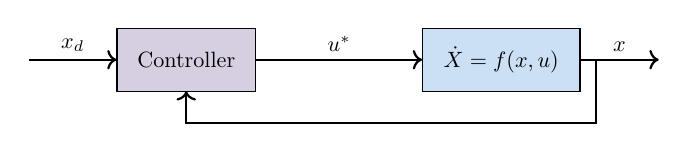
\begin{tikzpicture}[scale=0.8, transform shape]
    \node[draw, minimum width=2.2cm, minimum height=1cm, fill=nyuheader!50] (ctrl) at (0,0) {Controller};
    \node[draw, minimum width=2.5cm, minimum height=1cm, fill=brightblue!20] (sys) at (5,0) {$\dot{X} = f(x,u)$};
    
    \draw[->, thick] (-2.5,0) -- (ctrl) node[midway, above] {$x_d$};
    \draw[->, thick] (ctrl) -- (sys) node[midway, above] {$u^*$};
    \draw[->, thick] (sys) -- (7.5,0) node[midway, above] {$x$};
    
    \draw[->, thick] (6.5,0) -- (6.5,-1) -- (0,-1) -- (0,-0.5);
\end{tikzpicture}
\end{center}

\end{frame}

% ============================================================
\begin{frame}{Control Design Approach}

\textbf{Lyapunov-Based Control Design Steps:}

\vspace{0.5cm}

\begin{enumerate}
    \item Choose a Lyapunov candidate $V(x)$
    
    \vspace{0.4cm}
    
    \item Compute $\dot{V}(x, u)$
    
    \vspace{0.4cm}
    
    \item Design $u$ to make $\dot{V} \leq 0$ (or $< 0$)
\end{enumerate}

\end{frame}

% ============================================================
\begin{frame}{Example: Lyapunov Controller Design}

\textbf{System:}

\vspace{0.4cm}

\begin{equation*}
\ddot{x} + \dot{x}^2 + x^3 = u
\end{equation*}

\vspace{0.5cm}

\textbf{Goal:} Design $u$ such that $x \to 0$ as $t \to \infty$

\vspace{0.5cm}

\textbf{Choose Lyapunov function:}

\vspace{0.3cm}

\begin{equation*}
V(x) = \frac{1}{2}\dot{x}^2 + \frac{1}{4}x^4
\end{equation*}

\end{frame}

% ============================================================
\begin{frame}{Computing $\dot{V}$ for Control Design}

\textbf{Time derivative:}

\vspace{0.5cm}

\begin{align*}
\dot{V}(x) &= \ddot{x} \cdot \dot{x} + \dot{x} \cdot x^3 \\[0.3cm]
&= \dot{x}(\ddot{x} + x^3) \\[0.3cm]
&= \dot{x}(u - \dot{x}^2)
\end{align*}

\vspace{0.5cm}

Now we need to choose $u$ to make $\dot{V} < 0$.

\end{frame}

% ============================================================
\begin{frame}{Controller Selection}

\textbf{Choose:}

\vspace{0.5cm}

\begin{equation*}
u^* = \dot{x}^2 + x^2 - \dot{x}
\end{equation*}

\vspace{0.5cm}

\textbf{Then:}

\vspace{0.3cm}

\begin{equation*}
\dot{V} = \dot{x}(\dot{x}^2 + x^2 - \dot{x} - \dot{x}^2) = \dot{x} \cdot x^2 - \dot{x}^2
\end{equation*}

\end{frame}

% ============================================================
\begin{frame}{Closed-Loop System}

With control $u^* = \dot{x}^2 + x^2 - \dot{x}$, the closed-loop system becomes:

\vspace{0.5cm}

\begin{equation*}
\ddot{x} + \dot{x} + x^3 = 0
\end{equation*}

\vspace{0.5cm}

\begin{block}{Result}
This system is \textbf{globally asymptotically stable} by Lyapunov analysis!
\end{block}

\end{frame}

% ============================================================
% SECTION: ROBOT APPLICATION
% ============================================================
\begin{frame}{Application: Holonomic Robot Control}

\textbf{Euler-Lagrange Equations:}

\vspace{0.5cm}

\begin{equation*}
M(q)\ddot{q} + C(q, \dot{q})\dot{q} + G(q) = \tau
\end{equation*}

\vspace{0.5cm}

where:

\vspace{0.3cm}

\begin{itemize}
    \item[\textbullet] $M(q)$: inertia matrix (positive definite)
    
    \vspace{0.3cm}
    
    \item[\textbullet] $C(q, \dot{q})$: Coriolis/centrifugal matrix
    
    \vspace{0.3cm}
    
    \item[\textbullet] $G(q)$: gravity vector
\end{itemize}

\end{frame}

% ============================================================
\begin{frame}{Key Property}

\textbf{Important Property:}

\vspace{0.5cm}

$\dot{M} - 2C$ is \textbf{skew-symmetric}:

\vspace{0.5cm}

\begin{equation*}
x^T(\dot{M} - 2C)x = 0 \quad \forall x
\end{equation*}

\vspace{0.5cm}

This property is crucial for Lyapunov-based stability proofs in robot control.

\end{frame}

% ============================================================
\begin{frame}{PD + Gravity Compensation Controller}

\textbf{Control Law:}

\vspace{0.5cm}

\begin{equation*}
\tau = -K_p q - K_d \dot{q} + G(q)
\end{equation*}

\vspace{0.5cm}

where $K_p, K_d$ are diagonal positive-definite gain matrices.

\end{frame}

% ============================================================
\begin{frame}{Lyapunov Function for Robot}

\textbf{Choose:}

\vspace{0.5cm}

\begin{equation*}
V = \frac{1}{2}\dot{q}^T M(q) \dot{q} + \frac{1}{2}q^T K_p q
\end{equation*}

\vspace{0.5cm}

\textbf{Verification:}

\vspace{0.3cm}

\begin{itemize}
    \item[\textbullet] $V(0,0) = 0$ \quad \checkmark
    
    \vspace{0.3cm}
    
    \item[\textbullet] $V > 0$ for $(q, \dot{q}) \neq 0$ \quad \checkmark
\end{itemize}

\vspace{0.3cm}

(Since $M$ and $K_p$ are positive definite)

\end{frame}

% ============================================================
\begin{frame}{Time Derivative}

\textbf{Computing $\dot{V}$:}

\vspace{0.5cm}

\begin{equation*}
\dot{V} = \frac{1}{2}\dot{q}^T \dot{M} \dot{q} + \dot{q}^T M \ddot{q} + \dot{q}^T K_p q
\end{equation*}

\vspace{0.5cm}

After substituting closed-loop dynamics:

\vspace{0.3cm}

\begin{equation*}
\dot{V} = \frac{1}{2}\dot{q}^T (\dot{M} - 2C) \dot{q} - \dot{q}^T K_d \dot{q}
\end{equation*}

\end{frame}

% ============================================================
\begin{frame}{Stability Proof}

Using skew-symmetry of $(\dot{M} - 2C)$:

\vspace{0.5cm}

\begin{equation*}
\boxed{\dot{V} = -\dot{q}^T K_d \dot{q} \leq 0}
\end{equation*}

\vspace{0.5cm}

\begin{block}{Conclusion}
The robot system is \textbf{globally asymptotically stable}: $q, \dot{q} \to 0$
\end{block}

\end{frame}

% ============================================================
% SUMMARY
% ============================================================
\begin{frame}{Summary: Key Takeaways}

\begin{itemize}
    \item[\textbullet] Nonlinear systems have multiple equilibria with local stability
    
    \vspace{0.35cm}
    
    \item[\textbullet] Phase portraits visualize 2D system behavior
    
    \vspace{0.35cm}
    
    \item[\textbullet] Eigenvalues classify stability: $\text{Re}(\lambda) < 0 \Rightarrow$ stable
    
    \vspace{0.35cm}
    
    \item[\textbullet] Lyapunov: $V > 0$, $\dot{V} \leq 0$ $\Rightarrow$ stable
    
    \vspace{0.35cm}
    
    \item[\textbullet] $\dot{V} < 0$ $\Rightarrow$ asymptotically stable
    
    \vspace{0.35cm}
    
    \item[\textbullet] Lyapunov functions enable controller design
\end{itemize}

\end{frame}

% ============================================================
\begin{frame}{Connection to Next Lectures}

\begin{center}
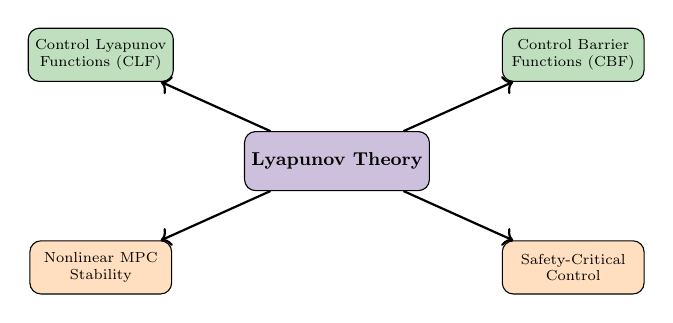
\begin{tikzpicture}[scale=0.75, transform shape]
    \node[draw, fill=nyupurple!30, rounded corners, minimum width=2.8cm, minimum height=1cm, font=\small\bfseries] (lyap) at (0,0) {Lyapunov Theory};
    
    \node[draw, fill=accentgreen!25, rounded corners, minimum width=2.4cm, minimum height=0.9cm, font=\scriptsize, align=center] (clf) at (-4,1.8) {Control Lyapunov\\Functions (CLF)};
    \node[draw, fill=accentgreen!25, rounded corners, minimum width=2.4cm, minimum height=0.9cm, font=\scriptsize, align=center] (cbf) at (4,1.8) {Control Barrier\\Functions (CBF)};
    \node[draw, fill=accentorange!25, rounded corners, minimum width=2.4cm, minimum height=0.9cm, font=\scriptsize, align=center] (nmpc) at (-4,-1.8) {Nonlinear MPC\\Stability};
    \node[draw, fill=accentorange!25, rounded corners, minimum width=2.4cm, minimum height=0.9cm, font=\scriptsize, align=center] (safe) at (4,-1.8) {Safety-Critical\\Control};
    
    \draw[->, thick] (lyap) -- (clf);
    \draw[->, thick] (lyap) -- (cbf);
    \draw[->, thick] (lyap) -- (nmpc);
    \draw[->, thick] (lyap) -- (safe);
\end{tikzpicture}
\end{center}

\vspace{0.3cm}

\textbf{Next:} NMPC with safety constraints via Control Barrier Functions.

\end{frame}

% ============================================================
% END SLIDE
% ============================================================
{
\setbeamertemplate{footline}{}
\begin{frame}[plain]
\begin{center}
\vspace{3cm}

{\Huge\bfseries End of Lecture 5}

\vspace{1.5cm}

{\Large Questions?}

\vspace{2cm}

{\normalsize Dr.\ Aliasghar Arab}

{\small NYU Tandon School of Engineering}
\end{center}
\end{frame}
}

\end{document}
